\documentclass[9pt]{beamer}
\usetheme{Madrid}
\usefonttheme{serif}

\usepackage{fontspec}
% надёжный шрифт с кириллицей (работает в Overleaf)
\setmainfont{Libertinus Serif}[Ligatures=TeX]
\setsansfont{Libertinus Sans}[Ligatures=TeX]
\newfontfamily\cyrillicfont{Libertinus Serif}
\newfontfamily\cyrillicfontsf{Libertinus Sans}
\usepackage{polyglossia}
\setmainlanguage{russian}
\setotherlanguage{english}

\usepackage{amsmath}
\usepackage{amsfonts}
\usepackage{amssymb}
\usepackage{graphicx}
\usepackage{microtype}

\usepackage{xcolor}
\usepackage{pifont}
\usepackage{tikz}
\newcommand{\plus}{\tikz[baseline=(X.base)] \node[fill=green!65!black, rounded corners=2pt, inner sep=2pt] (X) {\color{white}\ding{51}};}
\newcommand{\minus}{\tikz[baseline=(X.base)] \node[fill=red!70!black,   rounded corners=2pt, inner sep=2pt] (X) {\color{white}\ding{55}};}

\DeclareMathOperator{\sen}{sen}
% \DeclareMathOperator{\tg}{tg}

\setbeamertemplate{caption}[numbered]

% --- Информация о презентации ---
\author[Автор]{Чиняев Владимир Николаевич}
\title{Задача перехода в линейном приближении \\ (компланарный случай)}
\newcommand{\coursename}{Введение в маневрирование} % <-- Поставь здесь нужное название курса
\setbeamertemplate{navigation symbols}{} 
\institute[]{Московский физико технический институт} 
\date{30 сентября 2025 г.} 

\bibliographystyle{apalike}

% --- Кастомная нижняя синяя полоска: курс слева, номер слайда справа ---
\setbeamertemplate{footline}{
  \leavevmode%
  \begin{beamercolorbox}[wd=\paperwidth,ht=2ex,dp=1ex]{palette primary}
    \hspace{0.4cm}\usebeamerfont{footline}\coursename\hfill\usebeamerfont{footline}\insertframenumber\hspace{0.4cm}
  \end{beamercolorbox}%
}

% Чтобы убрать лишние отступы в footer-шрифте (опционально)
\setbeamerfont{footline}{size=\small}

\begin{document}

\begin{frame}
\titlepage
\end{frame}

\begin{frame}{Условия выхода на целевую орбиту}
\begin{gather*}
    \sum_{j=1}^{N} \Bigl( \Delta V_{rj} \sin \phi_j + 2 \Delta V_{tj} \cos \phi_j \Bigl) = V_0 \Delta e_x, \\
    \sum_{j=1}^{N} \Bigl( -\Delta V_{rj} \cos \phi_j + 2 \Delta V_{tj} \sin \phi_j \Bigl) = V_0 \Delta e_y, \\
    \sum_{j=1}^{N} 2 \Delta V_{tj} = V_0 \Delta a, \\
    \sum_{j=1}^{N} (2 \Delta V_{rj} (1 - \cos \phi_j) + \Delta V_{tj} (-3 \phi_i + 4 \sin \phi_j)) = V_0 \Delta t, \\
    \sum_{j=1}^{N} -\Delta V_{zj} \sin \phi_j = 0, \\
    \sum_{j=1}^{N} \Delta V_{zj} \cos \phi_j = V_0 \Delta i.
\end{gather*}
\end{frame}

\begin{frame}{Лагранжиан задачи}
\begin{equation*}
    \begin{aligned}
        L &= \sum_{j=1}^N \sqrt{\Delta V_{rj}^2 + \Delta V_{tj}^2 + \Delta V_{zj}^2} - \\
        &- h_1 \sum_{j=1}^N \left( \Delta V_{rj} \sin \phi_j + 2 \Delta V_{tj} \cos \phi_j \right) + h_1 \Delta e_x - \\
        &- h_2 \sum_{j=1}^N \left(- \Delta V_{rj} \cos \phi_j + 2 \Delta V_{tj} \sin \phi_j \right) + h_2 \Delta e_y - \\
        &- h_3 \sum_{j=1}^N \left( 2 \Delta V_{tj} \right) + h_3 \Delta a - \\
        &- h_4 \sum_{j=1}^N \left( 2 \Delta V_{rj} (1 - \cos \phi_j) + \Delta V_{tj} (-3 \phi_j + 4 \sin \phi_j) \right) + h_4 \Delta t - \\
        &- h_5 \sum_{j=1}^N \left( -\Delta V_{zj} \sin \phi_j \right) - \\
        &- h_6 \sum_{j=1}^N \left( \Delta V_{zj} \cos \phi_j \right) + h_6 \Delta i.
    \end{aligned}
\end{equation*}
\end{frame}

\begin{frame}{Необходимые условия оптимальности}
Необходимые условия оптимальности:
\begin{equation*}
    \begin{aligned}
        \frac{\partial L}{\partial \Delta V_{rj}} &= \frac{\Delta V_{rj}}{\Delta V_j} - h_1 \sin \phi_j + h_2 \cos \phi_j - 2 h_4 (1 - \cos \phi_j) = 0, \\
        \frac{\partial L}{\partial \Delta V_{tj}} &= \frac{\Delta V_{tj}}{\Delta V_j} - 2 h_1 \cos \phi_j - 2 h_2 \sin \phi_j - 2 h_3 - h_4 (-3 \phi_j + 4 \sin \phi_j) = 0, \\
        \frac{\partial L}{\partial \Delta V_{zj}} &= \frac{\Delta V_{zj}}{\Delta V_j} + h_5 \sin \phi_j - h_6 \cos \phi_j = 0.
    \end{aligned}
\end{equation*}
\end{frame}

\begin{frame}{Радиальная компонента}
\begin{equation*}
    \begin{aligned}
        \frac{\Delta V_{rj}}{\Delta V_j} &= h_1 \sin \phi_j - h_2 \cos \phi_j + 2 h_4 - 2 h_4 \cos \phi_j = \\
        &= h_1 \sin \phi_j - (h_2 + 2 h_4) \cos \phi_j + 2 h_4 = \\
        & \vert \lambda_3 = h_1, \lambda_6 = h_4, \lambda_2 = h_2 + 2 h_4, \phi_j = \theta \vert \\
        &= \lambda_3 \sin \theta - \lambda_2 \cos \theta + 2 \lambda_6 = \\
        & \vert \frac{\lambda_2}{\sqrt{\lambda_2^2 + \lambda_3^2}} = \sin \theta_0, \frac{\lambda_3}{\sqrt{\lambda_2^2 + \lambda_3^2}} = \cos \theta_0 \vert \\
        &= \sqrt{\lambda_2^2 + \lambda_3^2} \sin (\theta - \theta_0) + 2 \lambda_6.
    \end{aligned}
\end{equation*}
Получаем:
\begin{equation*}
    \boxed{\frac{\Delta V_{rj}}{\Delta V_j} = \sqrt{\lambda_2^2 + \lambda_3^2} \sin (\theta - \theta_0) + 2 \lambda_6}
\end{equation*}
\end{frame}

\begin{frame}{Трансверсальная компонента}
\begin{equation*}
    \begin{aligned}
        \frac{\Delta V_{tj}}{\Delta V_j} &= 2 h_1 \cos \phi_j + 2 h_2 \sin \phi_j + 2 h_3 + h_4 (-3 \phi_j + 4 \sin \phi_j) = \\
        &= 2 h_1 \cos \phi_j + 2 h_2 \sin \phi_j + 2 h_3 - 3 h_4 \phi_j + 4 h_4 \sin \phi_j = \\
        &= 2 \left( h_1 \cos \phi_j + (h_2 + 4 h_4) \sin \phi_j \right) + 2 h_3 - 3 h_4 \phi_j = \\
        & \vert \lambda_3 = h_1,  \lambda_6 = h_4, \lambda_2 = h_2 + 2 h_4, \lambda_1 = h_3 \vert \\
        &= 2 \left( \lambda_3 \cos \theta + \lambda_2 \sin \theta \right) + 2 \lambda_1 - 3 \lambda_6 \theta = \\
        & \vert \frac{\lambda_2}{\sqrt{\lambda_2^2 + \lambda_3^2}} = \sin \theta_0, \frac{\lambda_3}{\sqrt{\lambda_2^2 + \lambda_3^2}} = \cos \theta_0 \vert \\
        &= 2 \lambda_1 + 2 \sqrt{\lambda_2^2 + \lambda_3^2} \cos (\theta - \theta_0) - 3 \lambda_6 \theta.
    \end{aligned}
\end{equation*}
Получаем:
\begin{equation*}
    \boxed{\frac{\Delta V_{tj}}{\Delta V_j} = 2 \lambda_1 + 2 \sqrt{\lambda_2^2 + \lambda_3^2} \cos (\theta - \theta_0) - 3 \lambda_6 \theta} 
\end{equation*}
\end{frame}

\begin{frame}{Нормальная компонента}
\begin{equation*}
    \begin{aligned}
        \frac{\Delta V_{zj}}{\Delta V_j} &= -h_5 \sin \phi_j + h_6 \cos \phi_j = \vert \lambda_4 = -h_5, \lambda_5 = h_6 \vert \\
        &= \lambda_4 \sin \theta + \lambda_5 \cos \theta = \\
        &= \frac{1}{\lambda_2^2 + \lambda_3^2} \left( \lambda_4 \sin \theta (\lambda_2^2 + \lambda_3^2) + \lambda_5 \cos \theta (\lambda_2^2 + \lambda_3^2) \right) = \\
        &= \frac{1}{\lambda_2^2 + \lambda_3^2} \bigl( \lambda_3^2 \lambda_4 \sin \theta - \lambda_2 \lambda_3 \lambda_4 \cos \theta - \lambda_2 \lambda_3 \lambda_5 \sin \theta + \lambda_2^2 \lambda_5 \cos \theta + \\ 
        & \quad \quad \quad \quad \quad + \lambda_2 \lambda_3 \lambda_4 \cos \theta + \lambda_2^2 \lambda_4 \sin \theta + \lambda_3^2 \lambda_5 \cos \theta + \lambda_2 \lambda_3 \lambda_5 \sin \theta \bigr) = \\
        &= \frac{\lambda_3 \lambda_4 - \lambda_2 \lambda_5}{\lambda_2^2 + \lambda_3^2} \left( \sin \theta \lambda_3 - \lambda_2 \cos \theta \right) + \frac{\lambda_2 \lambda_4 + \lambda_3 \lambda_5}{\lambda_2^2 + \lambda_3^2} \left( \cos \theta \lambda_3 + \lambda_2 \sin \theta \right) = \\
        &= \frac{\lambda_3 \lambda_4 - \lambda_2 \lambda_5}{\sqrt{\lambda_2^2 + \lambda_3^2}} \left( \sin \theta \cos \theta_0 - \sin \theta_0 \cos \theta \right) + \frac{\lambda_2 \lambda_4 + \lambda_3 \lambda_5}{\sqrt{\lambda_2^2 + \lambda_3^2}} \left( \cos \theta \cos \theta_0 + \sin \theta_0 \sin \theta \right) = \\
        &= \frac{\lambda_3 \lambda_4 - \lambda_2 \lambda_5}{\sqrt{\lambda_2^2 + \lambda_3^2}} \sin (\theta - \theta_0) + \frac{\lambda_2 \lambda_4 + \lambda_3 \lambda_5}{\sqrt{\lambda_2^2 + \lambda_3^2}} \cos (\theta - \theta_0).
    \end{aligned}
\end{equation*}
Получаем:
\begin{equation*}
    \boxed{\frac{\Delta V_{zj}}{\Delta V_j} = \frac{\lambda_3 \lambda_4 - \lambda_2 \lambda_5}{\sqrt{\lambda_2^2 + \lambda_3^2}} \sin (\theta - \theta_0) + \frac{\lambda_2 \lambda_4 + \lambda_3 \lambda_5}{\sqrt{\lambda_2^2 + \lambda_3^2}} \cos (\theta - \theta_0)}
\end{equation*}
\end{frame}

\begin{frame}{Система уравнений для базис вектора}
Получим выражение для $\theta_0$:
\begin{equation*}
    \text{tg } \theta_0 = \frac{\sin \theta_0}{\cos \theta_0} = \frac{\lambda_2}{\sqrt{\lambda_2^2 + \lambda_3^2}} \frac{\sqrt{\lambda_2^2 + \lambda_3^2}}{\lambda_3} = \frac{\lambda_2}{\lambda_3}.
\end{equation*}
Тогда система будет иметь вид:
\begin{equation*}
    \boxed{
    \begin{aligned}
        &\lambda = \sqrt{\lambda_2^2 + \lambda_3^2} \sin (\theta - \theta_0) + 2 \lambda_6, \\
        &\mu = 2 \lambda_1 + 2 \sqrt{\lambda_2^2 + \lambda_3^2} \cos (\theta - \theta_0) - 3 \lambda_6 \theta, \\
        &\nu = \frac{\lambda_3 \lambda_4 - \lambda_2 \lambda_5}{\sqrt{\lambda_2^2 + \lambda_3^2}} \sin (\theta - \theta_0) + \frac{\lambda_2 \lambda_4 + \lambda_3 \lambda_5}{\sqrt{\lambda_2^2 + \lambda_3^2}} \cos (\theta - \theta_0), \\
        &\text{tg } \theta_0 = \frac{\lambda_2}{\lambda_3}. 
    \end{aligned}
    }
\end{equation*}
В общем случае эти уравнения описывают спираль в пространстве $\lambda, \mu, \nu$ или циклоиду на плоскости $\mu, \lambda$. Если $\lambda_6 = 0$, то годограф базис-вектора может вырождаться в эллипс, окружность, отрезок или точку. 
\end{frame}

\begin{frame}{Необходимые условия оптимальности}
Лоуден показал, что для оптимальной траектории должны быть выполнены следующие необходимые условия \cite{Lawden_all}, \cite{Edelbaum_1}:
\begin{enumerate}
    \item Базис-вектор и его производные должны быть непрерывны всюду;
    \item В моменты, когда ДУ активна, вектор тяги должен быть сонаправлен с базис-вектором;
    \item Величина модуля базис-вектора $\mathbf{s}$ не должна превышать $1$;
    \item Производная вектора $\mathbf{s}$ по времени должна быть равной нулю во всех точках приложения импульсов.
\end{enumerate}
Из условия 3 следует, что $|\mathbf{s}|$ достигает своего максимального значения в моменты осуществления маневрирования. \\
Это означает, что у оптимального решения годограф базис-вектора не выходит за пределы сферы единичного радиуса (пространственная задача) или окружности единичного радиуса (плоская задача). Импульсы скорости оптимального решения прикладываются только в те моменты, когда годограф касается сферы (окружности).
\end{frame}

\begin{frame}{Компланарный переход}
Условия выхода на целевую орбиту:
\begin{gather*}
    \sum_{j=1}^{2} \Bigl( \Delta V_{rj} \sin \phi_j + 2 \Delta V_{tj} \cos \phi_j \Bigl) = V_0 \Delta e_x, \\
    \sum_{j=1}^{2} \Bigl( -\Delta V_{rj} \cos \phi_j + 2 \Delta V_{tj} \sin \phi_j \Bigl) = V_0 \Delta e_y, \\
    \sum_{j=1}^{2} 2 \Delta V_{tj} = V_0 \Delta a.
\end{gather*}

Уравнения для базис вектора:
\begin{gather*}
    \begin{aligned}
        &\lambda= \sqrt{\lambda_2^2 + \lambda_3^2} \sin (\theta - \theta_0), \\
        &\mu = 2 \lambda_1 + 2 \sqrt{\lambda_2^2 + \lambda_3^2} \cos (\theta - \theta_0), \\
        &\nu = 0, \\
        &\text{tg } \theta_0 = \frac{\lambda_2}{\lambda_3},
    \end{aligned}
\end{gather*}
где $\lambda_6 = 0$, так как решение задачи не зависит от времени; $\lambda_4 = \lambda_5 = 0$, так как задача в компланарной постановке.
\end{frame}

\begin{frame}{Типы оптимальных решений}
\begin{columns}[T,onlytextwidth]
  % левая колонка
  \begin{column}{0.50\textwidth}
    \begin{center}
        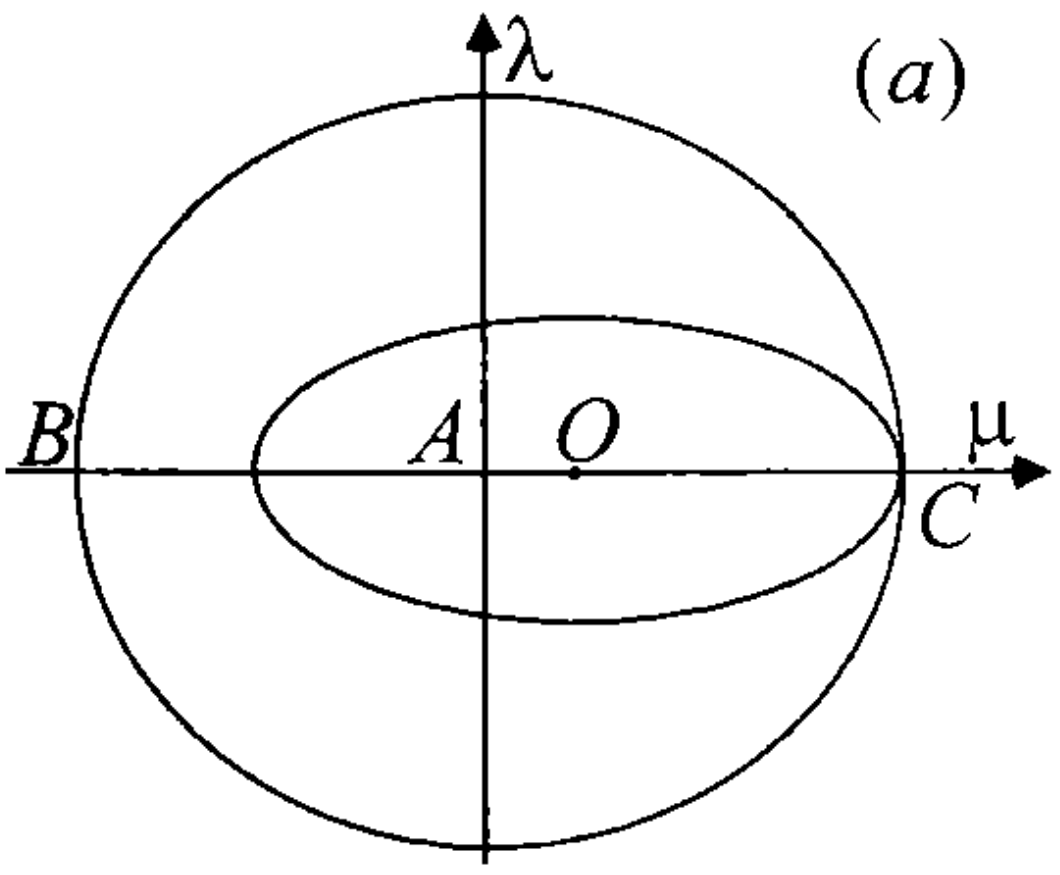
\includegraphics[height=0.4\textheight,keepaspectratio]{images/3/primer_a.png}
        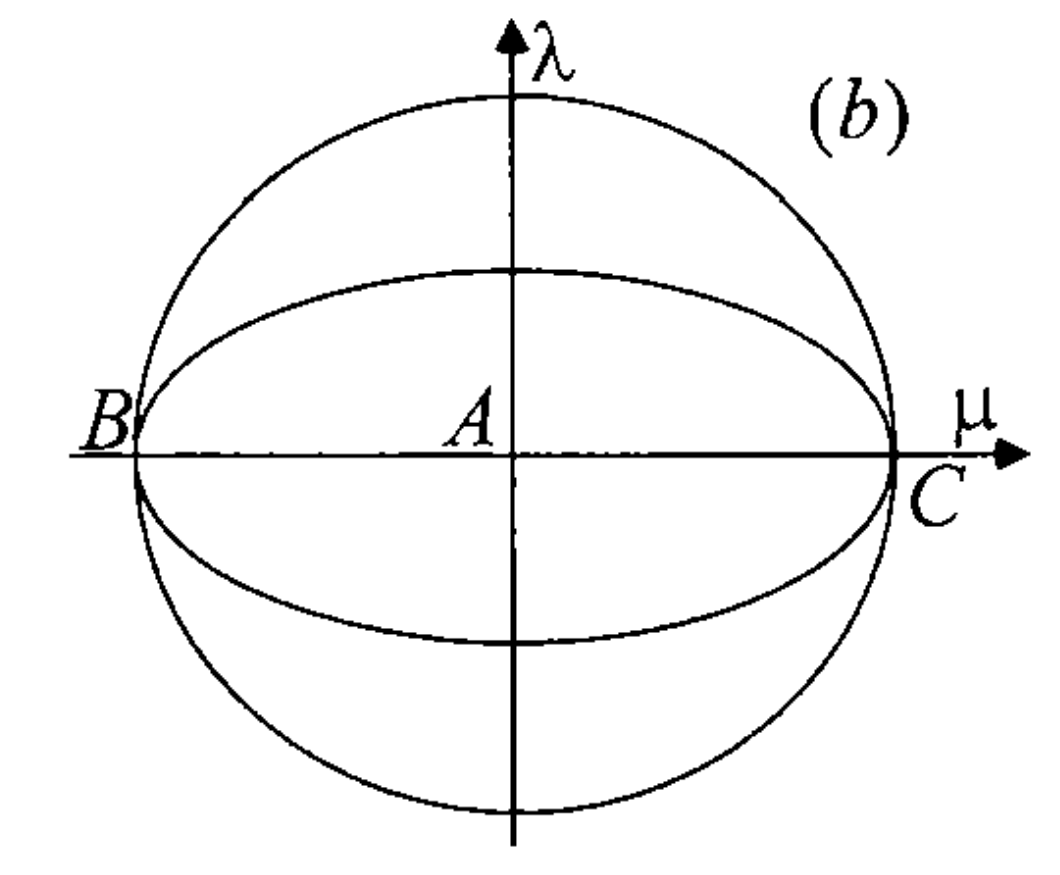
\includegraphics[height=0.43\textheight,keepaspectratio]{images/3/primer_b.png}
    \end{center}
  \end{column}

  % правая колонка
  \begin{column}{0.50\textwidth}
        \begin{itemize}
            \item На плоскости $\mu, \lambda$ годограф базис-вектора \textemdash\ эллипс, центр которого расположен на оси $\mu$, но смещён о начала системы координат; эллипс касается окружности единичного радиуса в точке С (рис. (а)), если центр смещён вправо, или в точке B, если эллипс смещён в противоположную сторону. 
            \item Годограф базис-вектора вырождается в точку, совпадающую с точкой пересечения окружности единичного радиуса оси $\mu$, это точки B или C.
            \item Годограф базис-вектора \textemdash\ эллипс с центром в начале системы координат, касающийся окружности в двух точках, это точки B и C (рис. (b)).
        \end{itemize}
  \end{column}
\end{columns}
\end{frame}

\begin{frame}{Касающиеся орбиты}
\begin{columns}[T,onlytextwidth]
  % левая колонка
  \begin{column}{0.50\textwidth}
    \begin{center}
        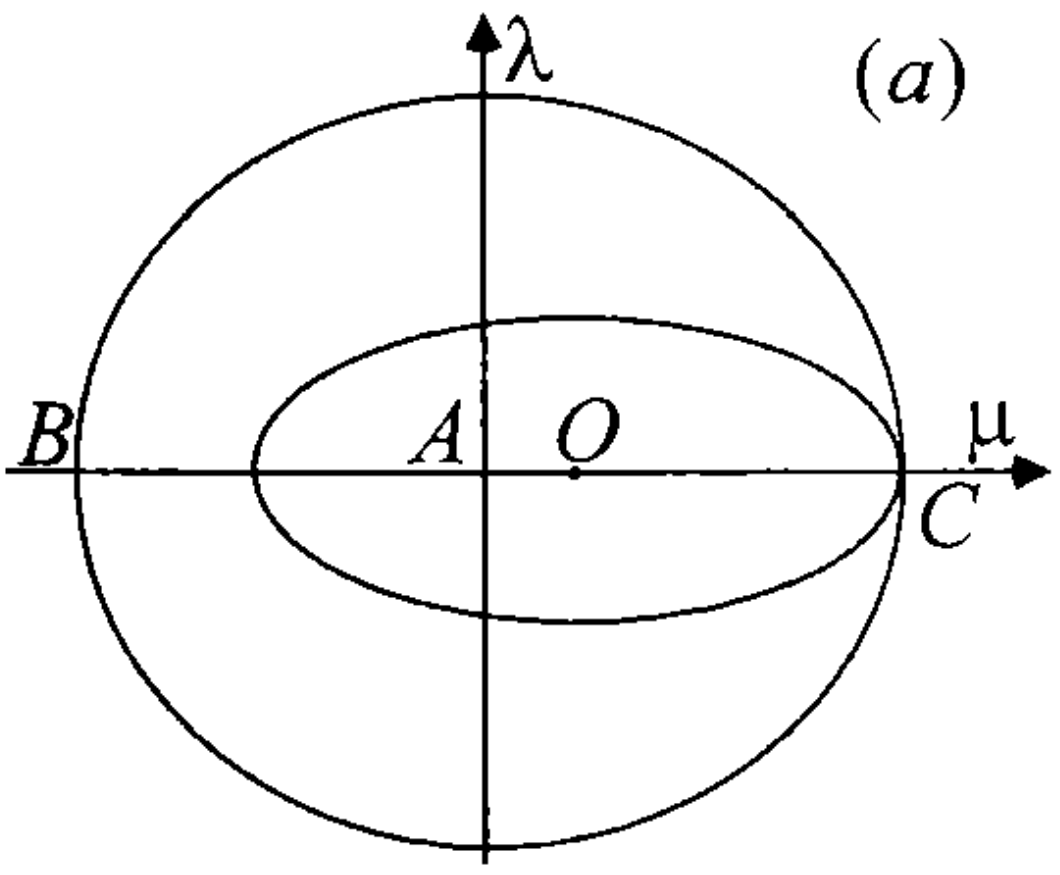
\includegraphics[height=0.4\textheight,keepaspectratio]{images/3/primer_a.png}
    \end{center}
    Если $\lambda_1 \neq 0$ и $\lambda_2^2 + \lambda_3^2 \neq 0$, то годограф базис-вектора \textemdash\ эллипс, смещённый относительно начала координат. Условия касания эллипсом окружности единичного радиуса:
    \begin{equation*}
        \left[
        \begin{aligned}
          2 \lambda_1 + 2 \sqrt{\lambda_2^2 + \lambda_3^2} &= 1, &\ &\text{если } \lambda_1 > 0,\\
          2 \lambda_1 - 2 \sqrt{\lambda_2^2 + \lambda_3^2} &= -1, &\ &\text{если } \lambda_1 < 0.
        \end{aligned}
        \right.
    \end{equation*}
  \end{column}

  % правая колонка
  \begin{column}{0.50\textwidth}
    Годограф касается окружности в одной точке на оси $\mu$ \textemdash\ $(\mu = 1; \lambda = 0)$. Оптимальное решение \textemdash\ один трансверсальный импульс в точке касания. Получаем:
    \begin{gather*}
        2 \Delta V_t = \Delta a, \\
        \Delta V_t = \frac{1}{2} \Delta a.
    \end{gather*}
    или
    \begin{equation*}
        \left\{
        \begin{aligned}
          2 \Delta V_t \cos \phi &= \Delta e_x, \\
          2 \Delta V_t \sin \phi &= \Delta e_y.
        \end{aligned}
        \right.
    \end{equation*}
    \begin{gather*}
        4 \Delta V_t^2 \cos^2 \phi + 4 \Delta V_t^2 \sin^2 \phi = \Delta e_x^2 + \Delta e_y^2, \\
        4 \Delta V_t^2 = \Delta e_x^2 + \Delta e_y^2, \\
        \Delta V_t = \frac{1}{2} \sqrt{\Delta e_x^2 + \Delta e_y^2} = \frac{1}{2} \Delta e.
    \end{gather*}
    Для касающихся орбит справедливо: $\boxed{\vert \Delta a \vert = \Delta e}$.
  \end{column}
\end{columns}
\end{frame}

\begin{frame}{Касающиеся орбиты}
\begin{center}
    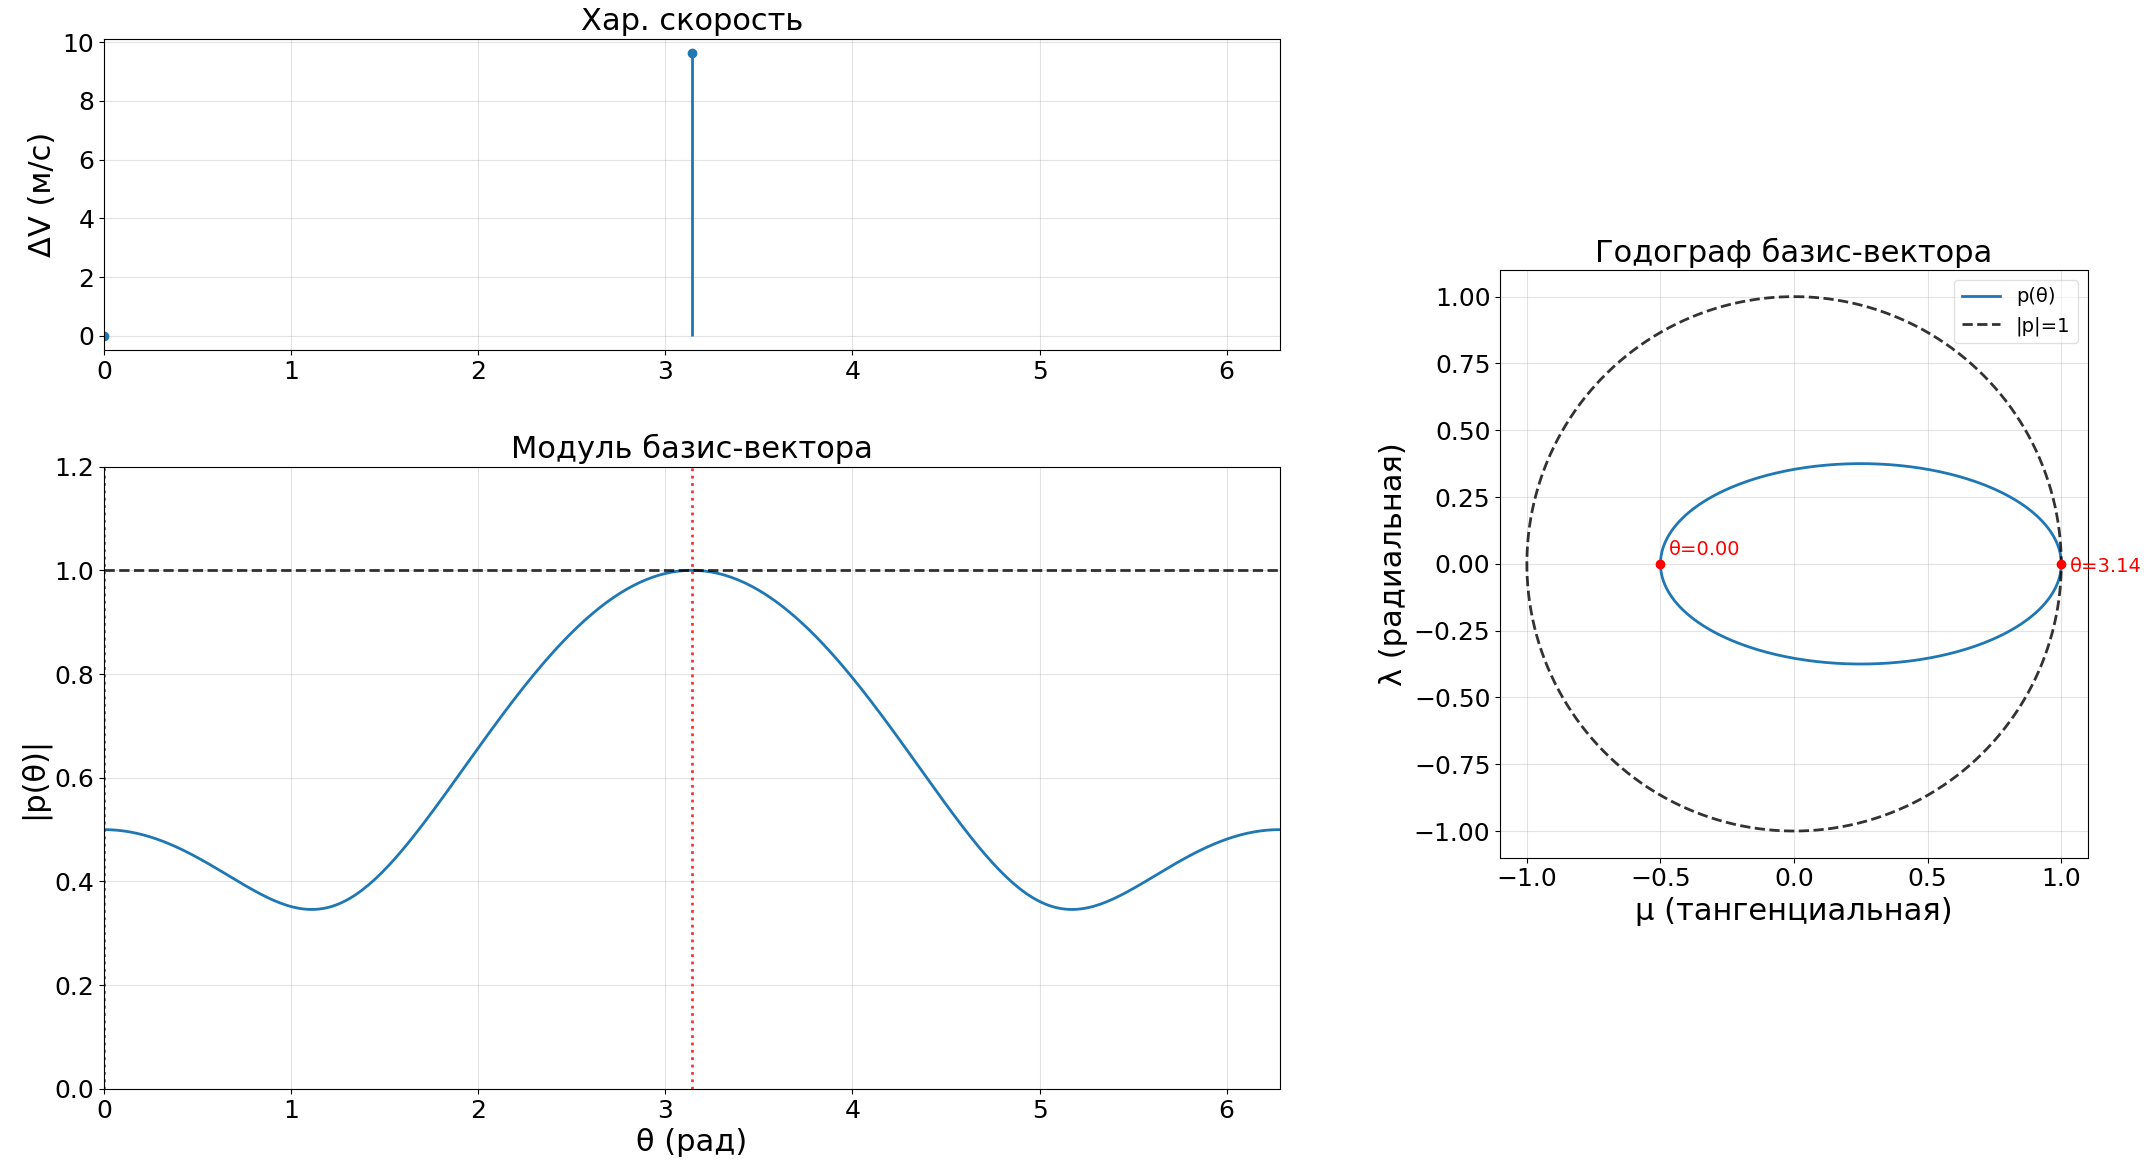
\includegraphics[height=0.7\textheight,keepaspectratio]{images/4/primer_tan_1.png}
\end{center}
\end{frame}

\begin{frame}{Касающиеся орбиты}
\begin{center}
    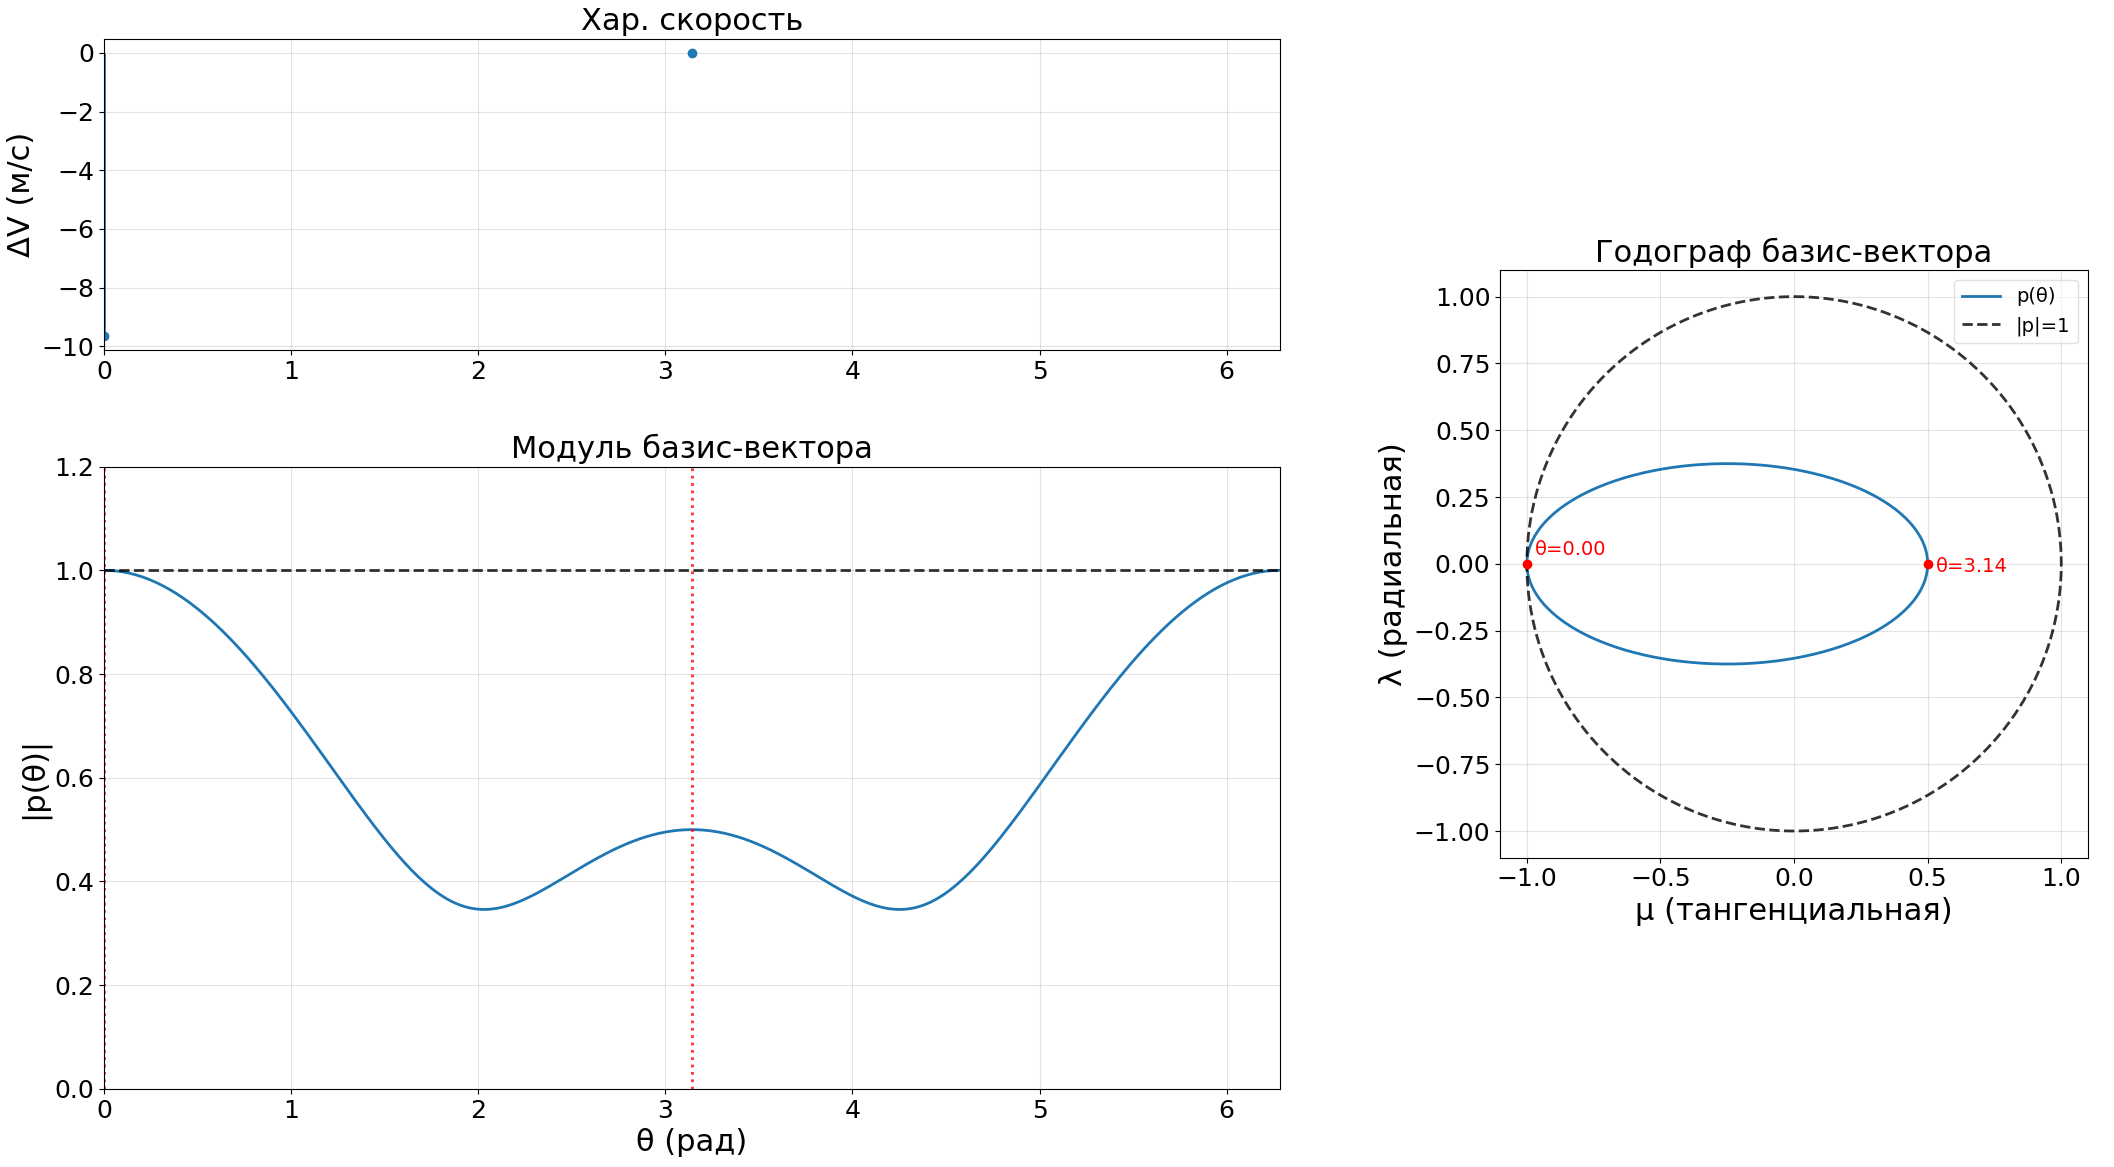
\includegraphics[height=0.7\textheight,keepaspectratio]{images/4/primer_tan_2.png}
\end{center}
\end{frame}

\begin{frame}{Непересекающиеся орбиты}
\begin{columns}[T,onlytextwidth]
  % левая колонка
  \begin{column}{0.50\textwidth}
    \begin{center}
        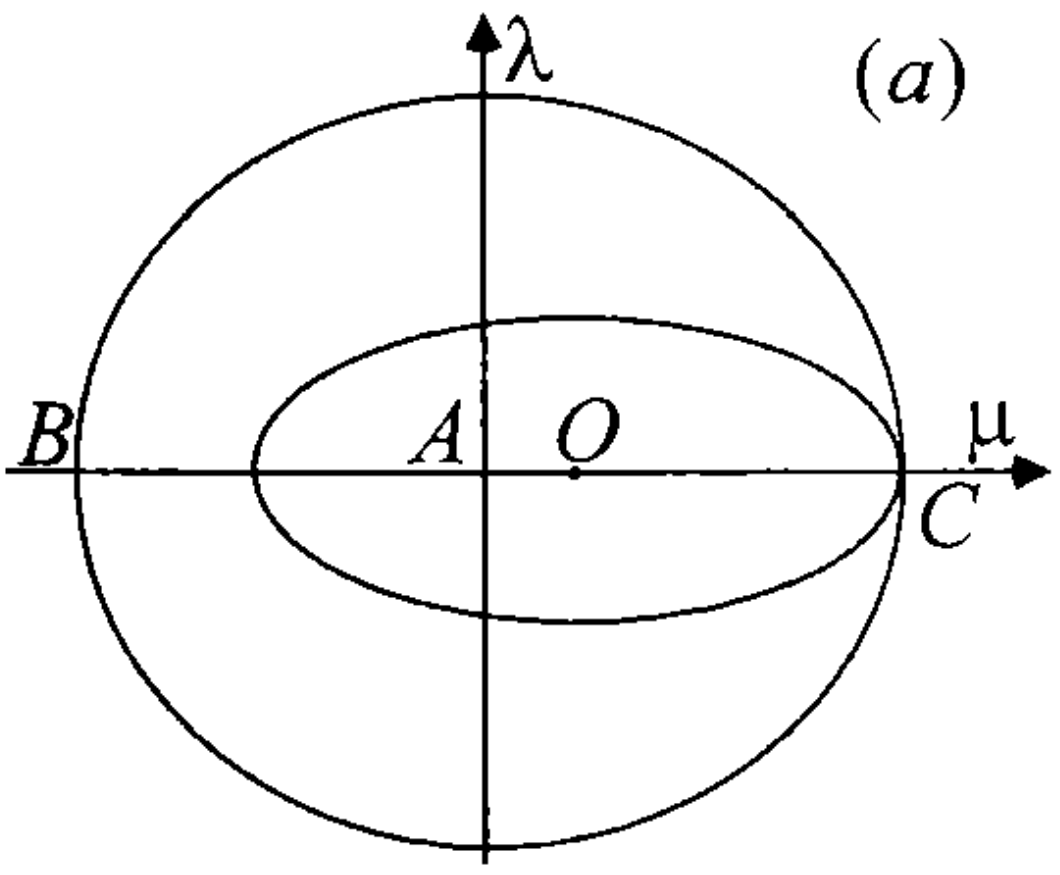
\includegraphics[height=0.4\textheight,keepaspectratio]{images/3/primer_a.png}
    \end{center}
    Эллипс вырождается в точку на единичной окружности, тогда $\lambda_2 = \lambda_3 = 0$ и $\lambda_1 = \pm \frac{1}{2}$. Получаем две точки на плоскости $(\mu, \lambda)$: $(1, 0)$ и $(-1, 0)$. Импульсы скорости трансверсальные, так как $\lambda = 0$. Все импульсы разгонные, если $\mu = 1$, или тормозные, если $\mu = -1$. Для такого типа переходов справедливо, что:
    \begin{equation*}
        \boxed{\vert \Delta a \vert > \Delta e}
    \end{equation*}
  \end{column}

  % правая колонка
  \begin{column}{0.50\textwidth}
    Cуммарная хар. скорость манёвра:
    \begin{equation*}
        \Delta V = \sum_{i=1}^2 \vert \Delta V_{ti} \vert = \frac{\vert \Delta a \vert}{2}.
    \end{equation*}
    Нет зависимости от угла приложения $\theta$, поэтому зафиксируем угол приложения первого импульса $\phi_1 = \phi_{1f}$. Получим систему:
    \begin{equation*}
        \left\{
        \begin{aligned}
          &2 \Delta V_{t1} \cos \phi_{1f} + 2 \Delta V_{t2} \cos \phi_{2} = \Delta e_x, \\
          &2 \Delta V_{t1} \sin \phi_{1f} + 2 \Delta V_{t2} \sin \phi_{2} = \Delta e_y, \\
          &2 \Delta V_{t1} + 2 \Delta V_{t2} = \Delta a.
        \end{aligned}
        \right.
    \end{equation*}
    Из последнего уравнения системы:
    \begin{equation*}
        \Delta V_{t2} = \frac{\Delta a}{2} - \Delta V_{t1}.
    \end{equation*}
  \end{column}
\end{columns}
\end{frame}

\begin{frame}{Непересекающиеся орбиты}
Преобразуем первые два уравнения системы:
\begin{equation*}
    \left\{
    \begin{aligned}
      &2 \Delta V_{t2} \cos \phi_{2} = \Delta e_x - 2 \Delta V_{t1} \cos \phi_{1f}, \\
      &2 \Delta V_{t2} \sin \phi_{2} = \Delta e_y - 2 \Delta V_{t1} \sin \phi_{1f}.
    \end{aligned}
    \right.
\end{equation*}
Возведём в квадрат и сложим:
\begin{align*}
    4 \Delta V_{t2}^2 &= \Delta e_x^2 + 4 \Delta V_{t1}^2 \cos^2 \phi_{1f} - 4 \Delta e_x \Delta V_{t1} \cos \phi_{1f} + \\ 
    &+ \Delta e_y^2 + 4 \Delta V_{t1}^2 \sin^2 \phi_{1f} - 4 \Delta e_y \Delta V_{t1} \sin \phi_{1f},
\end{align*}
\begin{gather*}
    4 \left( \frac{\Delta a^2}{4} + \Delta V_{t1}^2 - \Delta a \Delta V_{t1} \right) - 4 \Delta V_{t1}^2 = \Delta e_x^2 + \Delta e_y^2 - 4 \Delta V_{t1} \left( \Delta e_x \cos \phi_{1f} + \Delta e_y \sin \phi_{1f} \right), \\
    \Delta a^2 + 4 \Delta V_{t1}^2 - 4 \Delta a \Delta V_{t1} - 4 \Delta V_{t1}^2 = \Delta e^2 - 4 \Delta V_{t1} \left( \Delta e_x \cos \phi_{1f} + \Delta e_y \sin \phi_{1f} \right), \\
    4 \Delta V_{t1} \left( \Delta e_x \cos \phi_{1f} + \Delta e_y \sin \phi_{1f} - \Delta a \right) = \Delta e^2 - \Delta a^2, \\
    \Delta V_{t1} = \frac{\Delta e^2 - \Delta a^2}{4 \left( \Delta e_x \cos \phi_{1f} + \Delta e_y \sin \phi_{1f} - \Delta a \right)}, \\
    \text{tg } \phi_2 = \frac{\Delta e_y - 2 \Delta V_{t1} \sin \phi_{1f}}{\Delta e_x - 2 \Delta V_{t1} \cos \phi_{1f}}.
\end{gather*}
\end{frame}

\begin{frame}{Непересекающиеся орбиты}
Итоговые формулы оптимального маневрирования для случая непересекающихся орбит:
\begin{equation*}
\boxed{
    \begin{aligned}
        \Delta V_{t1} &= \frac{\Delta e^2 - \Delta a^2}{4 \left( \Delta e_x \cos \phi_{1f} + \Delta e_y \sin \phi_{1f} - \Delta a \right)}, \\
        \Delta V_{t2} &= \frac{\Delta a}{2} - \Delta V_{t1}, \\
        \text{tg } \phi_2 &= \frac{\Delta e_y - 2 \Delta V_{t1} \sin \phi_{1f}}{\Delta e_x - 2 \Delta V_{t1} \cos \phi_{1f}}, \\
        \text{Угол } &\phi_{1f} \text{ выбирается произвольно в диапазоне } (0; 2\pi].
    \end{aligned}
}
\end{equation*}
\end{frame}

\begin{frame}{Непересекающиеся орбиты}
\begin{center}
    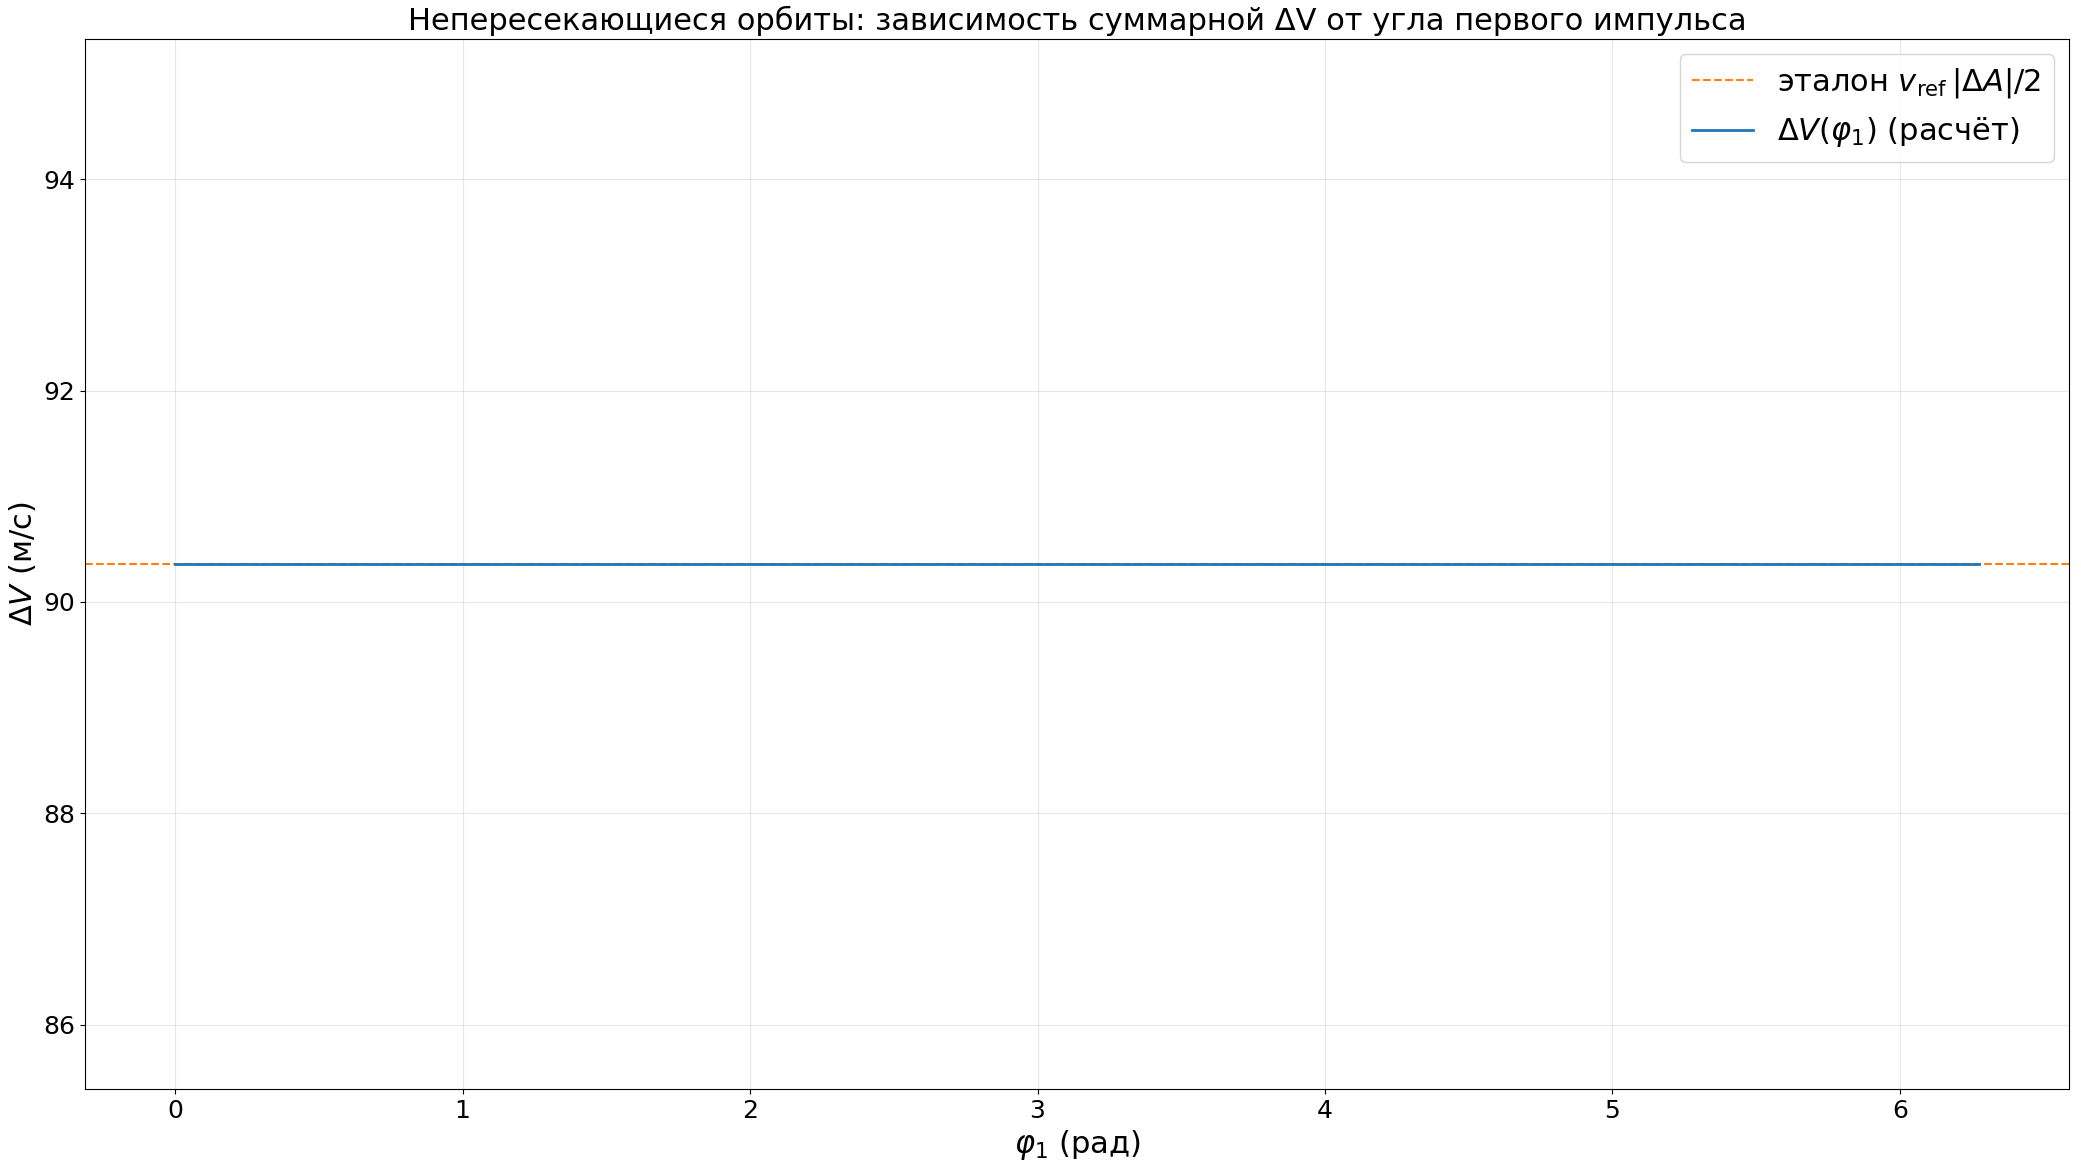
\includegraphics[height=0.7\textheight,keepaspectratio]{images/4/non_int_dv.png}
\end{center}
\end{frame}

\begin{frame}{Непересекающиеся орбиты}
\begin{center}
    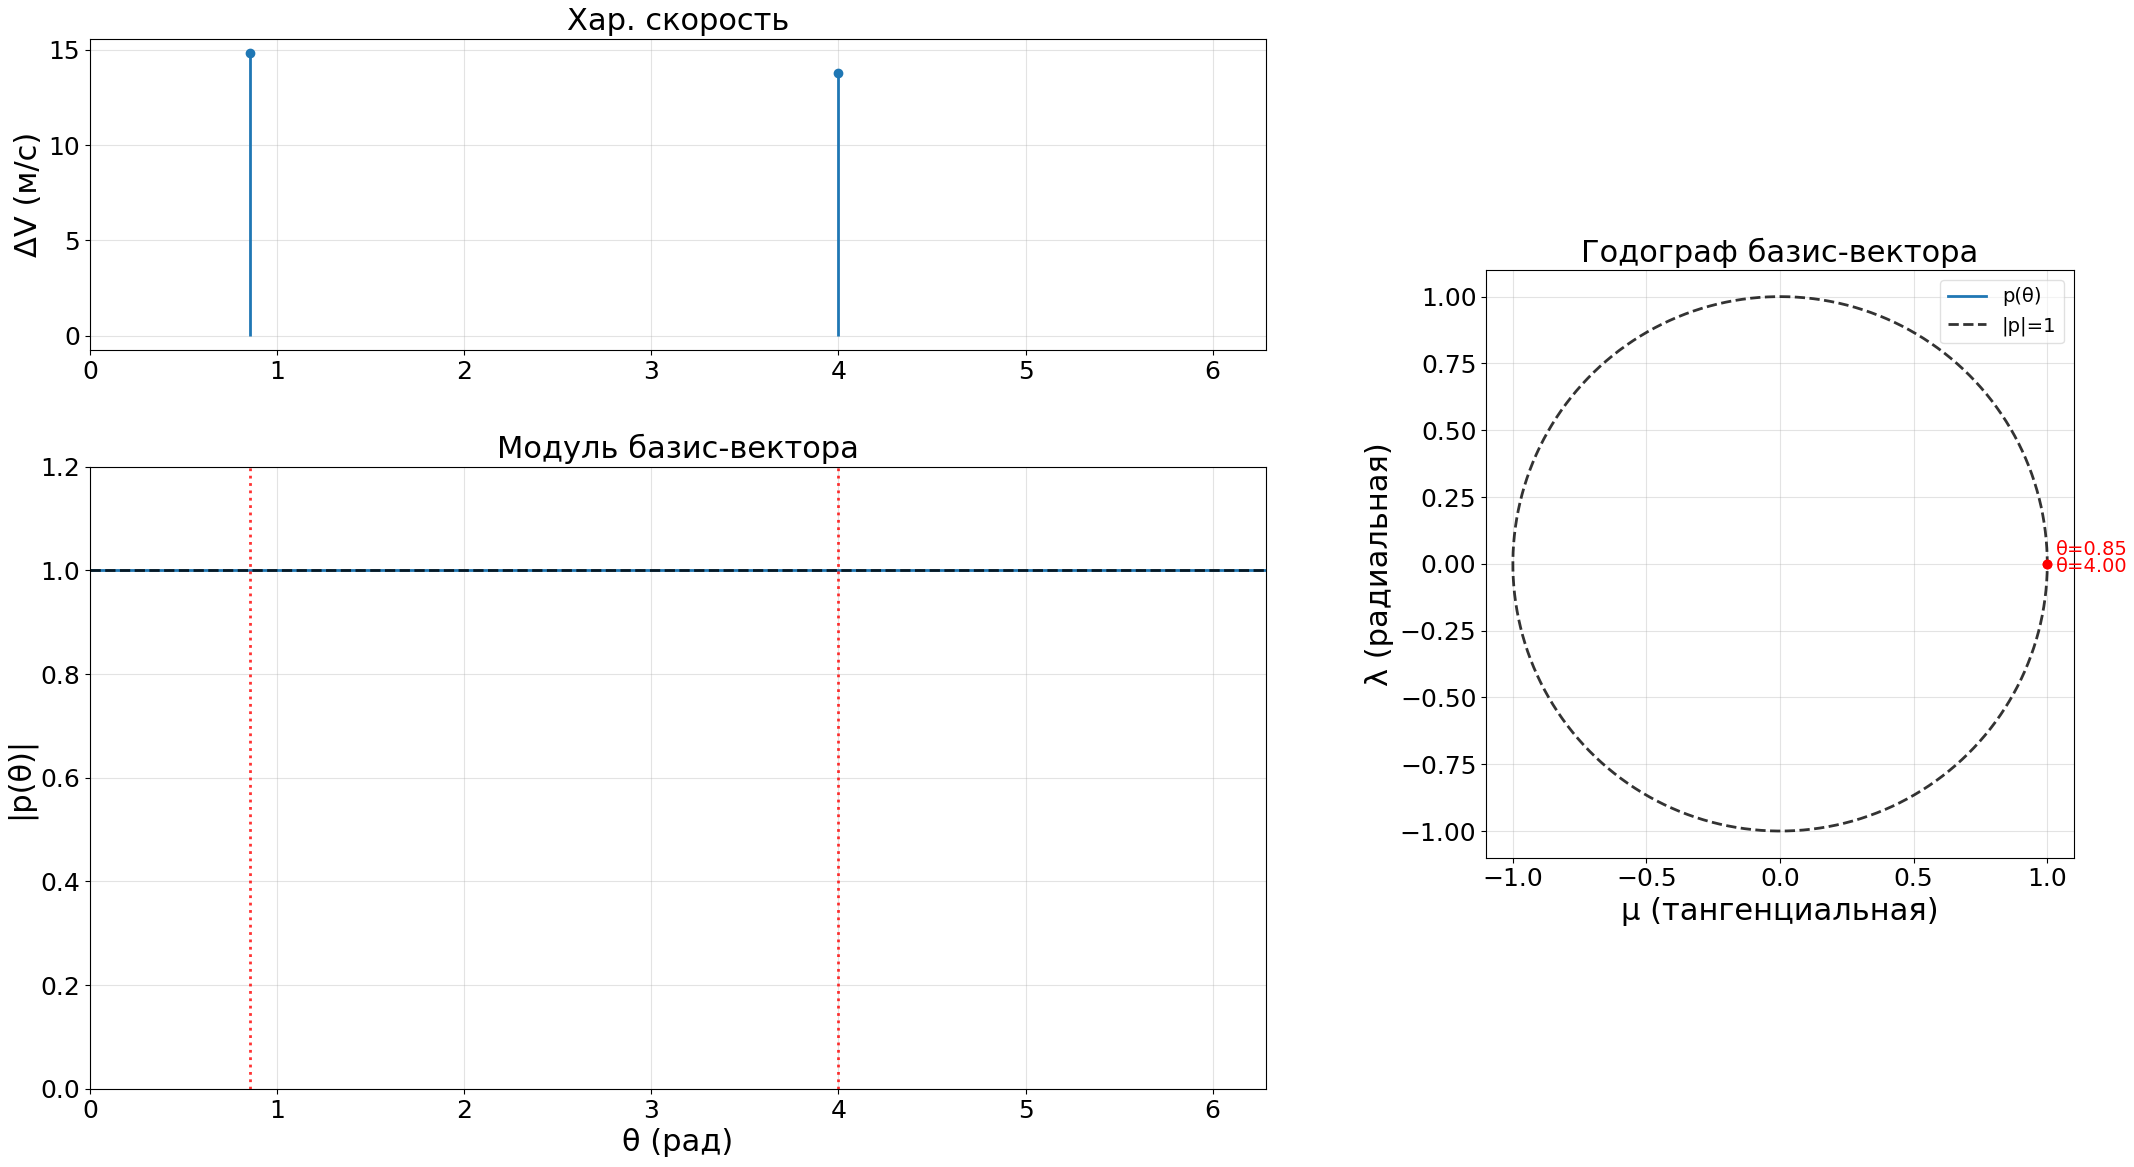
\includegraphics[height=0.7\textheight,keepaspectratio]{images/4/primer_non_int_1.png}
\end{center}
\end{frame}

\begin{frame}{Непересекающиеся орбиты}
\begin{center}
    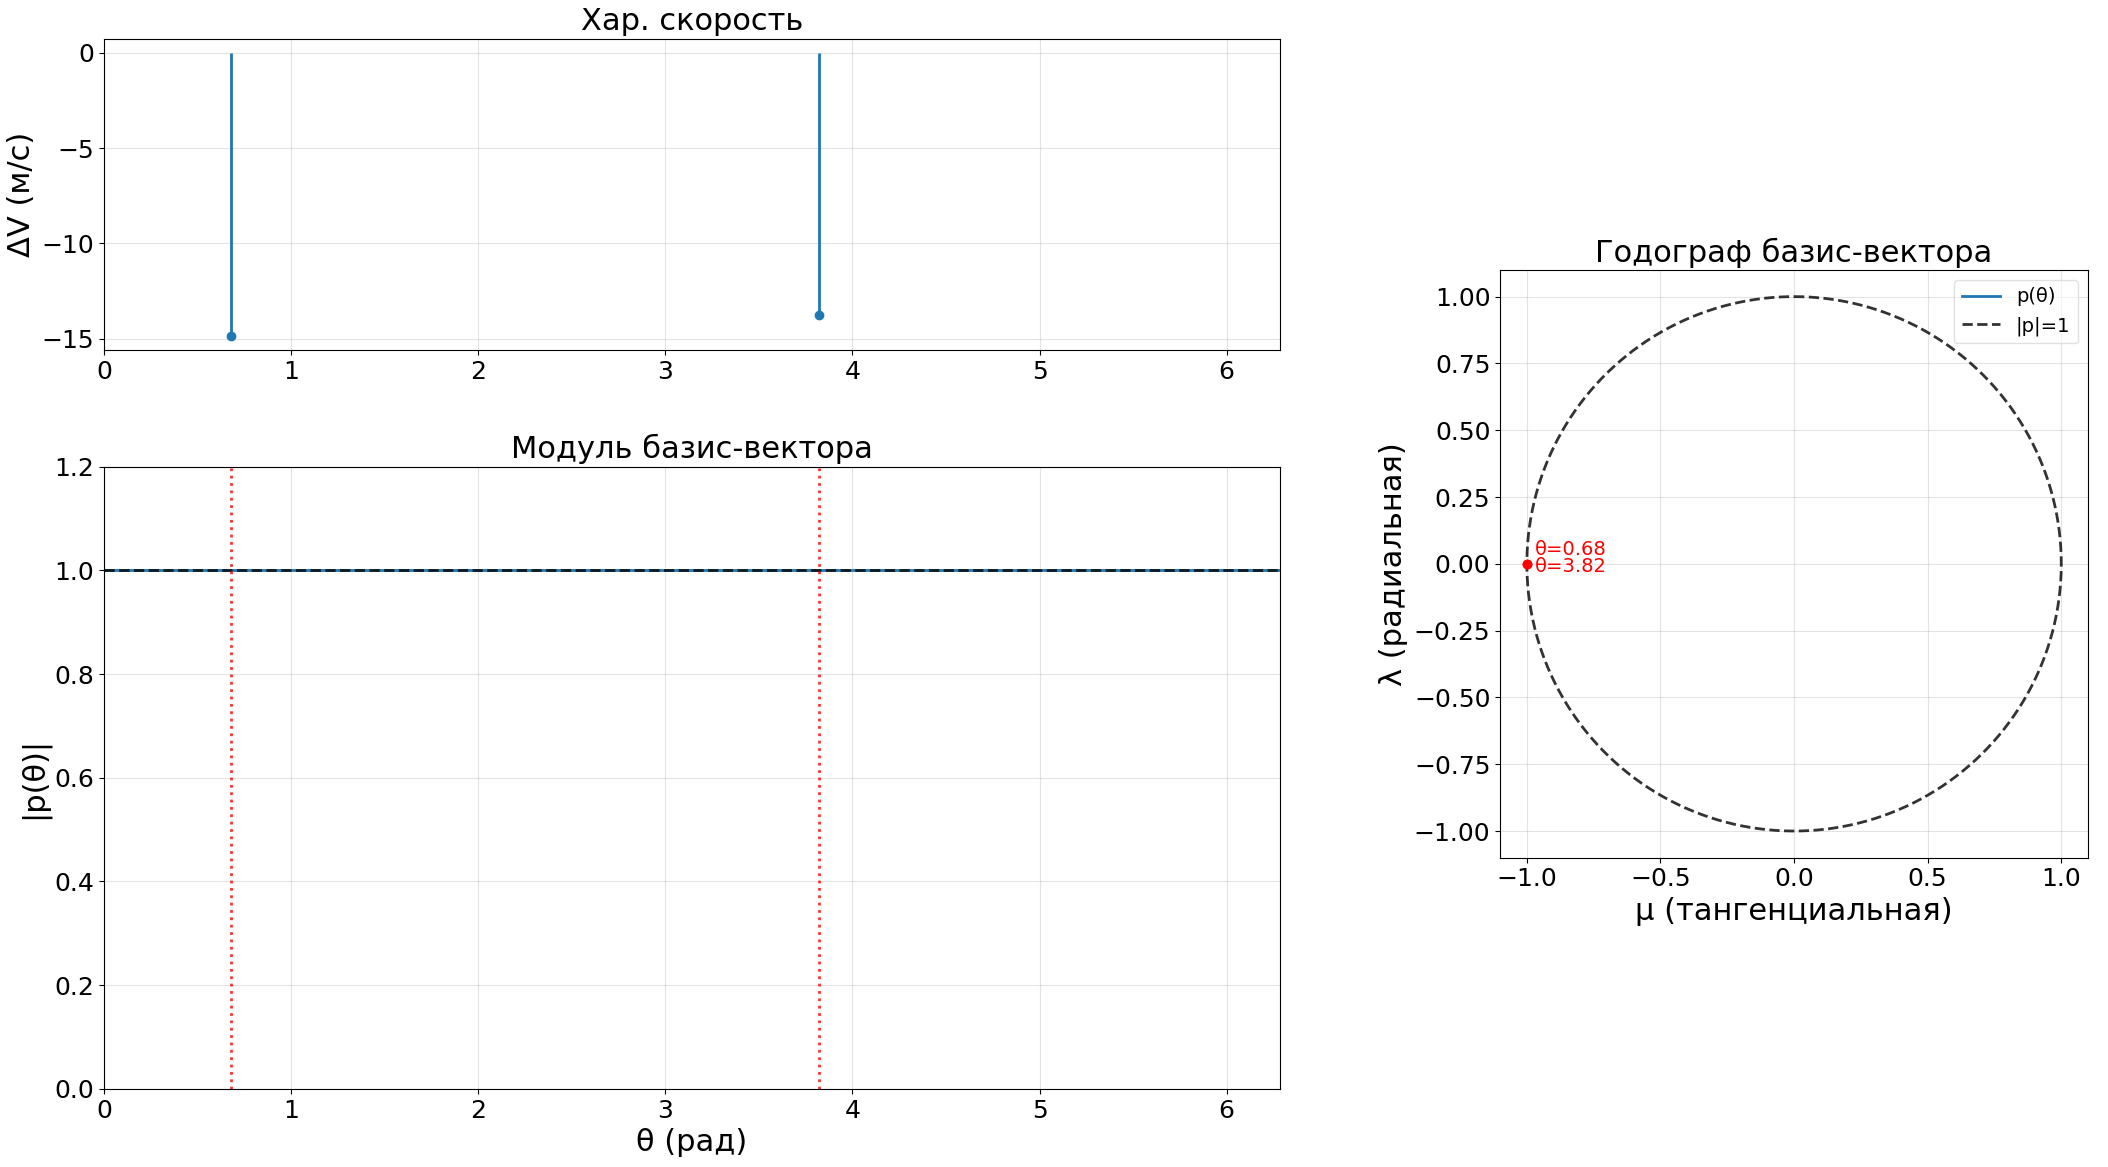
\includegraphics[height=0.7\textheight,keepaspectratio]{images/4/primer_non_int_2.png}
\end{center}
\end{frame}

\begin{frame}{Пересекающиеся орбиты}
\begin{columns}[T,onlytextwidth]
  % левая колонка
  \begin{column}{0.50\textwidth}
    \begin{center}
        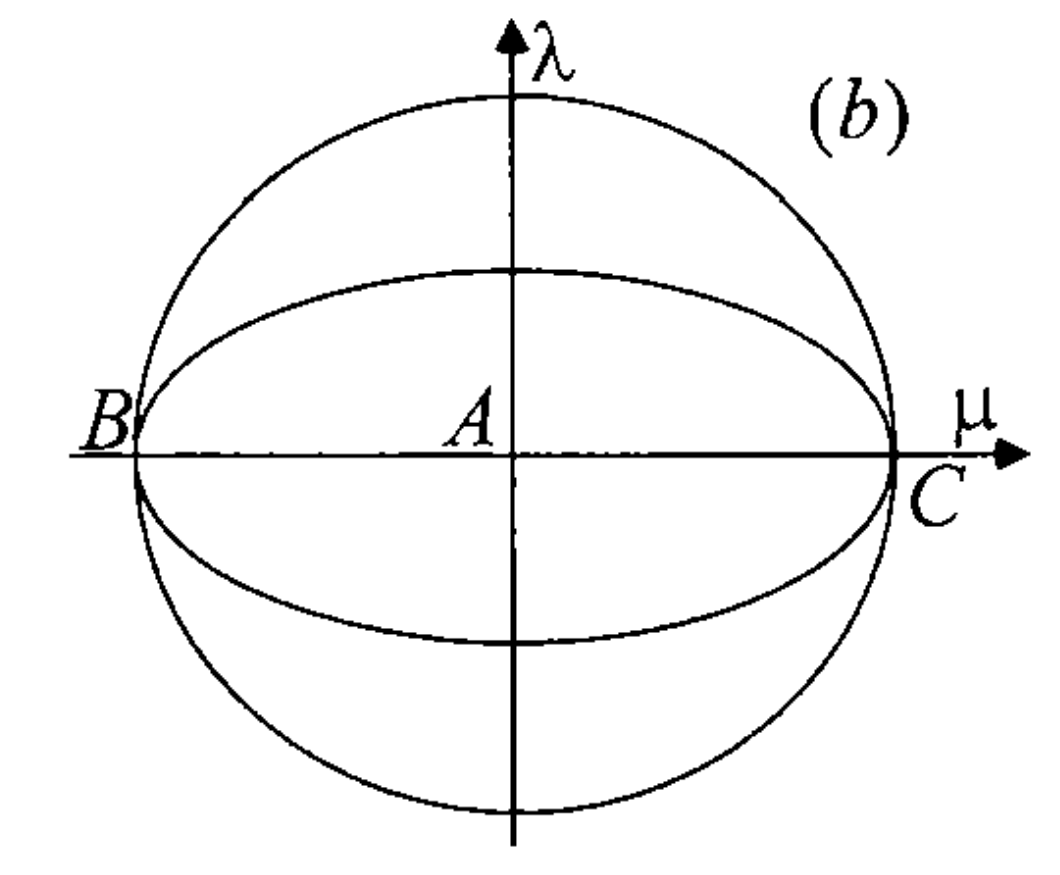
\includegraphics[height=0.35\textheight,keepaspectratio]{images/3/primer_b.png}
    \end{center}
    Годограф базис-вектора \textemdash\ эллипс с центром в начале координат, следовательно, $\sqrt{\lambda_2^2 + \lambda_3^2} = \frac{1}{2}$, $\lambda_1 = 0$. Получаем две точки на плоскости $(\mu, \lambda)$: $(1, 0)$ и $(-1, 0)$. Импульсы скорости трансверсальные, так как $\lambda = 0$. Углы приложения отличаются на половину витка, тогда пусть $\phi_2 = \phi_1 + \pi$ и
    \begin{align*}
        \cos (\phi_2) &= \cos (\phi_1 + \pi) = -\cos \phi_1, \\
        \sin (\phi_2) &= \sin (\phi_1 + \pi) = -\sin \phi_1.
    \end{align*}
  \end{column}

  % правая колонка
  \begin{column}{0.50\textwidth} 
    Снова рассмотрим знакомую систему:
    \begin{equation*}
        \left\{
        \begin{aligned}
          &2 \Delta V_{t1} \cos \phi_{1} + 2 \Delta V_{t2} \cos \phi_{2} = \Delta e_x, \\
          &2 \Delta V_{t1} \sin \phi_{1} + 2 \Delta V_{t2} \sin \phi_{2} = \Delta e_y, \\
          &2 \Delta V_{t1} + 2 \Delta V_{t2} = \Delta a.
        \end{aligned}
        \right.
    \end{equation*}
    С помощью выражений для углов, первые два уравнения системы можно преобразовать:
    \begin{equation*}
        \left\{
        \begin{aligned}
          &\Delta V_{t1} \cos \phi_{1} - \Delta V_{t2} \cos \phi_{1} = \frac{1}{2} \Delta e_x, \\
          &\Delta V_{t1} \sin \phi_{1} - \Delta V_{t2} \sin \phi_{1} = \frac{1}{2} \Delta e_y.
        \end{aligned}
        \right.
    \end{equation*}
    \begin{equation*}
        \left\{
        \begin{aligned}
          &\cos \phi_{1} \left( \Delta V_{t1} - \Delta V_{t2} \right) = \frac{1}{2} \Delta e_x, \\
          & \sin \phi_{1} \left( \Delta V_{t1} - \Delta V_{t2} \right) = \frac{1}{2} \Delta e_y.
        \end{aligned}
        \right.
    \end{equation*}
  \end{column}
\end{columns}
\end{frame}

\begin{frame}{Пересекающиеся орбиты}
Возведём уравнения системы в квадрат и сложим их:
\begin{gather*}
    \left( \Delta V_{t1} - \Delta V_{t2} \right)^2 = \frac{1}{4} \Delta e_x^2 + \frac{1}{4} \Delta e_y^2 = \frac{1}{4} \Delta e^2, \\
    \Delta V_{t1} - \Delta V_{t2} = \frac{1}{2} \Delta e.
\end{gather*}
Используем третье уравнение системы:
\begin{gather*}
    \Delta V_{t1} = \frac{1}{2} \Delta a - \Delta V_{t2} \quad \Rightarrow \quad \frac{1}{2} \Delta a - \Delta V_{t2} - \Delta V_{t2} = \frac{1}{2} \Delta e \quad \Rightarrow \quad \Delta V_{t2} = \frac{1}{4} (\Delta a - \Delta e),
\end{gather*}
\begin{equation*}
    \Delta V_{t1} = \frac{1}{2} \Delta a - \frac{1}{4} \Delta a + \frac{1}{4} \Delta e = \frac{1}{4} (\Delta a + \Delta e).
\end{equation*}
Поделив первые два уравнения системы, можно получить следующее выражение:
\begin{equation*}
    \text{tg }  \phi_1 = \text{tg }  \phi_e = \frac{\Delta e_y}{\Delta e_x}.
\end{equation*}
\end{frame}

\begin{frame}{Пересекающиеся орбиты}
Итоговые формулы оптимального маневрирования для случая пересекающихся орбит:
\begin{equation*}
\boxed{
    \begin{aligned}
         \Delta V_{t1} &= \frac{1}{4} (\Delta a + \Delta e), \\
         \Delta V_{t2} &= \frac{1}{4} (\Delta a - \Delta e), \\
         \phi_1 = &\phi_e, \quad \phi_2 = \phi_e + \pi, \\
         \text{tg }  &\phi_1 = \frac{\Delta e_y}{\Delta e_x}.
    \end{aligned}
}
\end{equation*}
\end{frame}

\begin{frame}{Пересекающиеся орбиты}
\begin{center}
    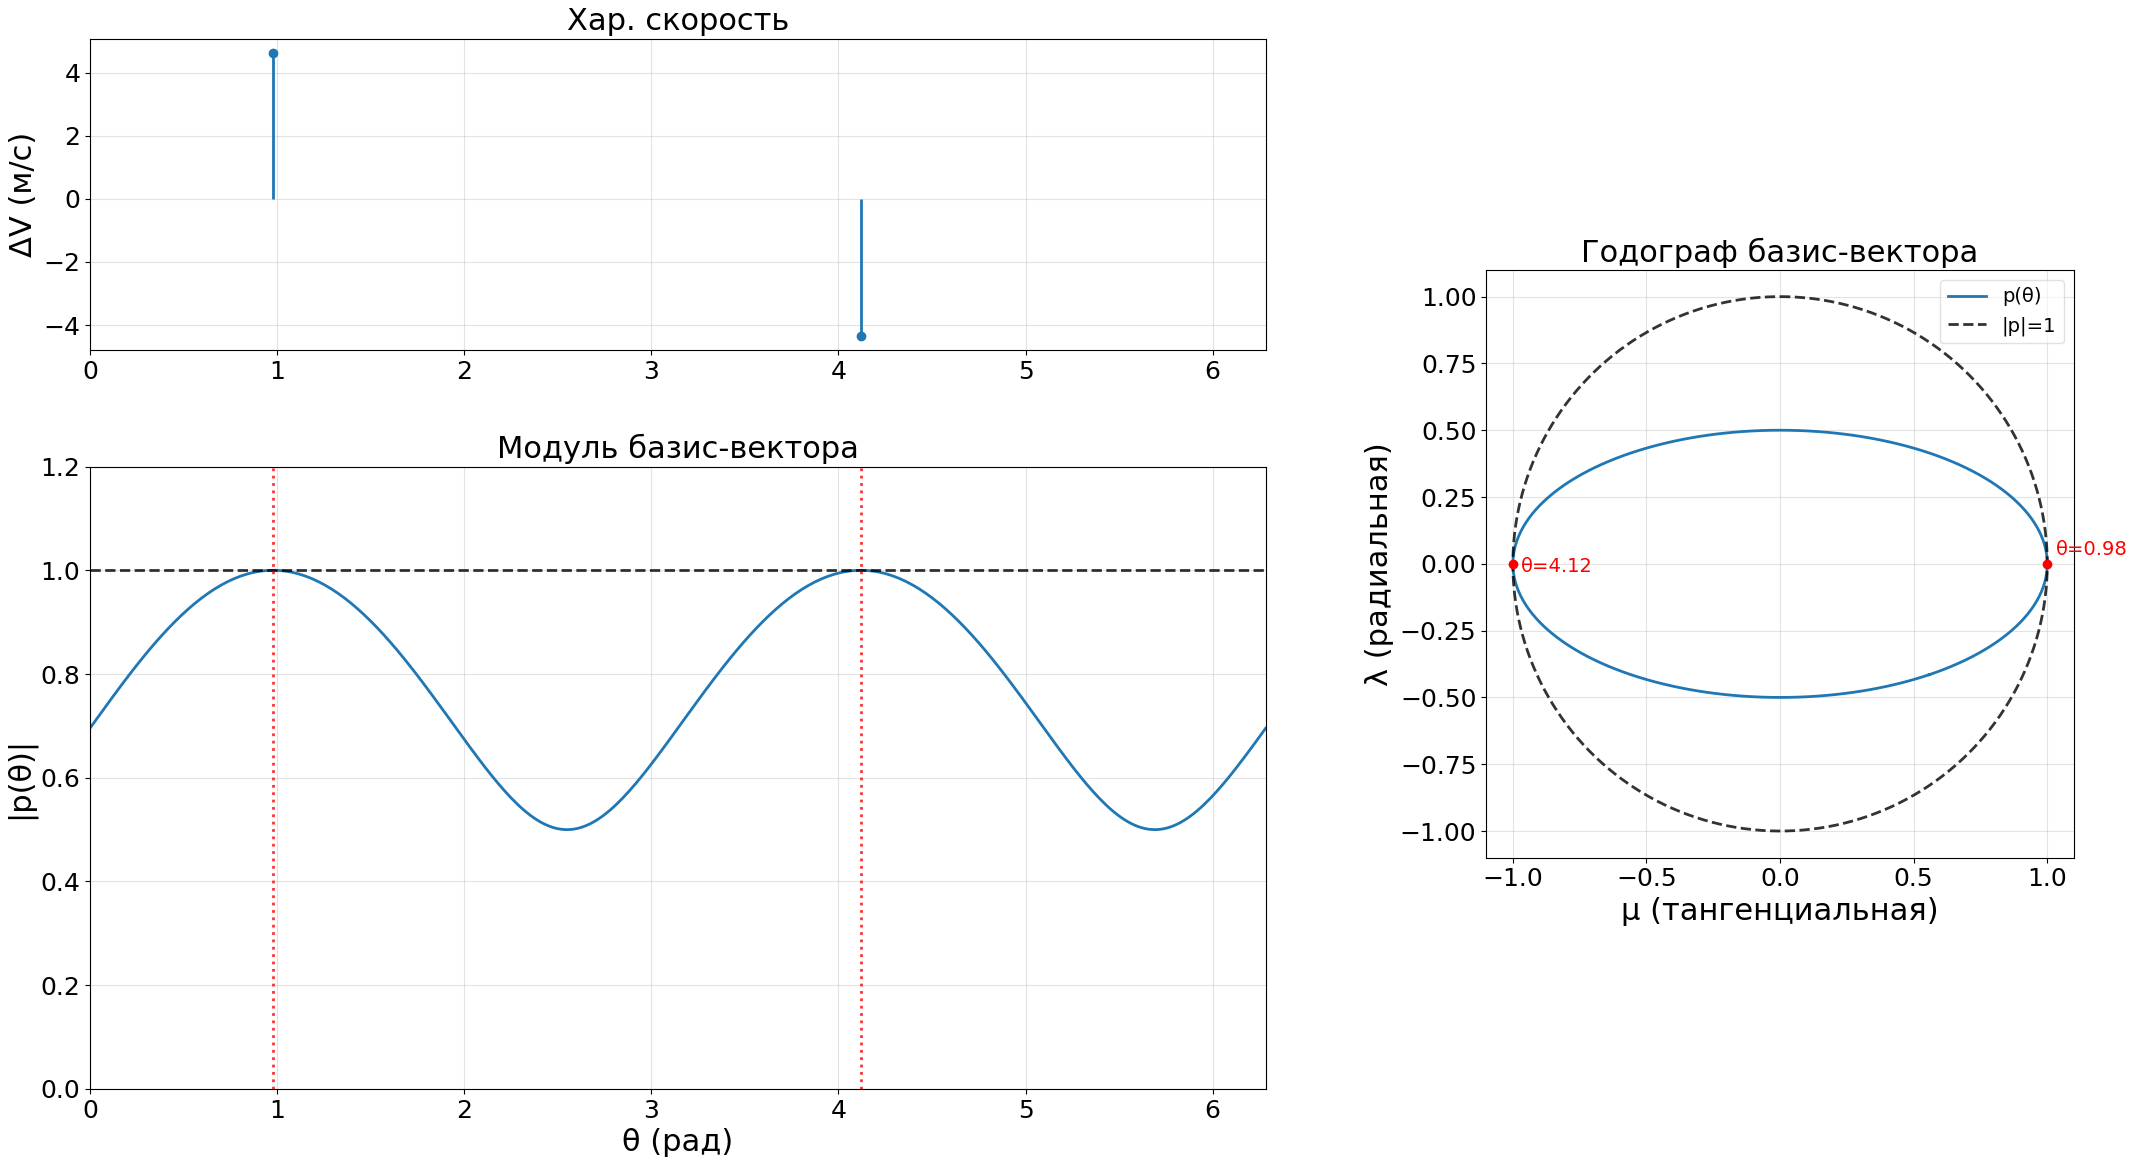
\includegraphics[height=0.7\textheight,keepaspectratio]{images/4/primer_int.png}
\end{center}
\end{frame}

\begin{frame}[allowframebreaks]{Источники}
  \begin{thebibliography}{9}
    \bibitem{Baranov}
    Баранов А. А. Маневрирование космических аппаратов в окрестности круговой орбиты //М.: Спутник. – 2016.

    \bibitem{Lawden_all}
    Лоуден Д. Ф. Оптимальные траектории для космической навигации. – 1966.
  
    \bibitem{Edelbaum_1}
    Edelbaum T. N., Gobetz F. W., Washington M. Minimum-impulse time-free transfer between elliptic orbits. – 1966. – №. NASA-CR-636.
    
  \end{thebibliography}
\end{frame}

\end{document}